\begin{frame}
  \frametitle{Ingresos del GNC \\ \small{Fuente: MHCP - CARF}}
  \begin{center}
    \scalebox{0.75}{
      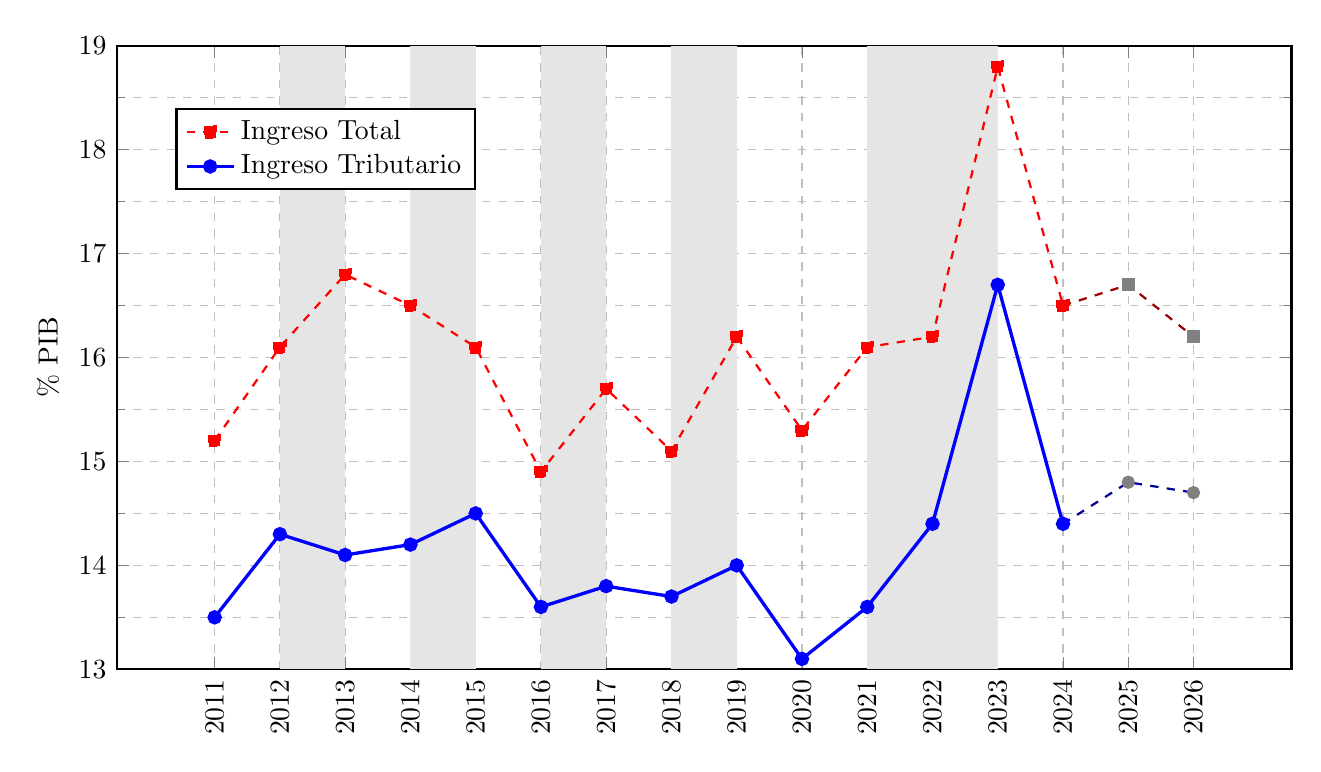
\begin{tikzpicture}
      \begin{axis}[
          width=16.5cm,
          height=9.5cm,
          ylabel={\% PIB},
          % ticks manuales para incluir 2025 y 2026
          xtick={7,...,22},
          xticklabels={2011,2012,2013,2014,2015,2016,2017,2018,2019,2020,2021,2022,2023,2024,2025,2026},
          x tick label style={rotate=90, anchor=east},
          ymin=13,
          ymax=19,
          grid=major,
          grid=both,
          grid style=dashed,
          minor y tick num=1,
          legend style={at={(0.05,0.9)}, anchor=north west},
          legend cell align={left},
          thick
      ]

      % Sombras de reformas tributarias
      %\draw [fill=gray!20, draw=none] (axis cs:06,13) rectangle (axis cs:07,19);
      \draw [fill=gray!20, draw=none] (axis cs:08,13) rectangle (axis cs:09,19);
      \draw [fill=gray!20, draw=none] (axis cs:10,13) rectangle (axis cs:11,19);
      \draw [fill=gray!20, draw=none] (axis cs:12,13) rectangle (axis cs:13,19);
      \draw [fill=gray!20, draw=none] (axis cs:14,13) rectangle (axis cs:15,19);
      \draw [fill=gray!20, draw=none] (axis cs:17,13) rectangle (axis cs:18,19);
      \draw [fill=gray!20, draw=none] (axis cs:18,13) rectangle (axis cs:19,19);

      % Ingreso Total (histórico)
      \addplot[
          mark=square*,
          dashed,
          red
      ] coordinates {
          (7,15.2) (8,16.1) (9,16.8) (10,16.5) (11,16.1) (12,14.9) (13,15.7) (14,15.1)
          (15,16.2) (16,15.3) (17,16.1) (18,16.2) (19,18.8) (20,16.5)
      };

      % Ingreso Tributario (histórico)
      \addplot[
          mark=*,
          very thick,
          blue
      ] coordinates {
          (7,13.5) (8,14.3) (9,14.1) (10,14.2) (11,14.5) (12,13.6) (13,13.8) (14,13.7)
          (15,14.0) (16,13.1) (17,13.6) (18,14.4) (19,16.7) (20,14.4)
      };

      % Proyecciones Ingreso Total (línea punteada)
      \addplot[
          color=red!60!black,
          dashed
      ] coordinates {
          (20,16.5) (21,16.7) (22,16.2)
      };

      % Proyecciones Ingreso Tributario (línea punteada)
      \addplot[
          color=blue!60!black,
          dashed
      ] coordinates {
          (20,14.4) (21,14.8) (22,14.7)
      };

      % Puntos grises Ingreso Total
      \addplot[
          color=gray,
          mark=square*,
          only marks
      ] coordinates {
          (21,16.7) (22,16.2)
      };

      % Puntos grises Ingreso Tributario
      \addplot[
          color=gray,
          mark=*,
          only marks
      ] coordinates {
          (21,14.8) (22,14.7)
      };

      \legend{Ingreso Total, Ingreso Tributario}
      \end{axis}
      \end{tikzpicture}
    }
  \end{center}
\end{frame}
